\documentclass[crop=false, class=book]{standalone}

\usepackage{lipsum}

\begin{document}
	\section{findGSE}
	
	Il programma \textit{findGSE}~\cite{sun2017findGSE} ha come obiettivo principale la stima della lunghezza del genoma. Utilizzando le frequenze dei k-mer trovati nelle letture a disposizione, il programma compie una regressione non lineare dei dati utilizzando come funzione una \gls{snd} (\textit{skew normal distribution}~\cite{azzalini1985class,azzalini2005skew}).
	
	
	\subsection{Algoritmo}
	Nel programma viene assunto che le frequenze dei k-mer possano essere approssimate da una distribuzione normale asimmetrica $Y \sim \mathcal{SN}(\xi, \omega^2, \alpha)$. Presa in input la distribuzione delle frequenze dei k-mer (k-mer profile), l'algoritmo effettua la regressione determinando i quattro parametri che descrivono una distribuzione normale asimmetrica, la media $\xi$, la deviazione standard $\omega$, l'asimmetria $\alpha$ e un fattore di scala $s$. Ad ogni iterazione, il programma cerca di minimizzare l'errore tra i dati di input e la funzione stimata, in modo da approssimare il più possibile il k-mer profile reale. La figura~\vref{fig:findGSEfitting} mostra come viene effettuato iterativamente il fitting del k-mer profile utilizzando come funzione la suddetta distribuzione.
	
	\begin{figure}[h]
		\centering
		\subfloat[][\emph{Primo fitting dei dati dalle letture di input.}]
		{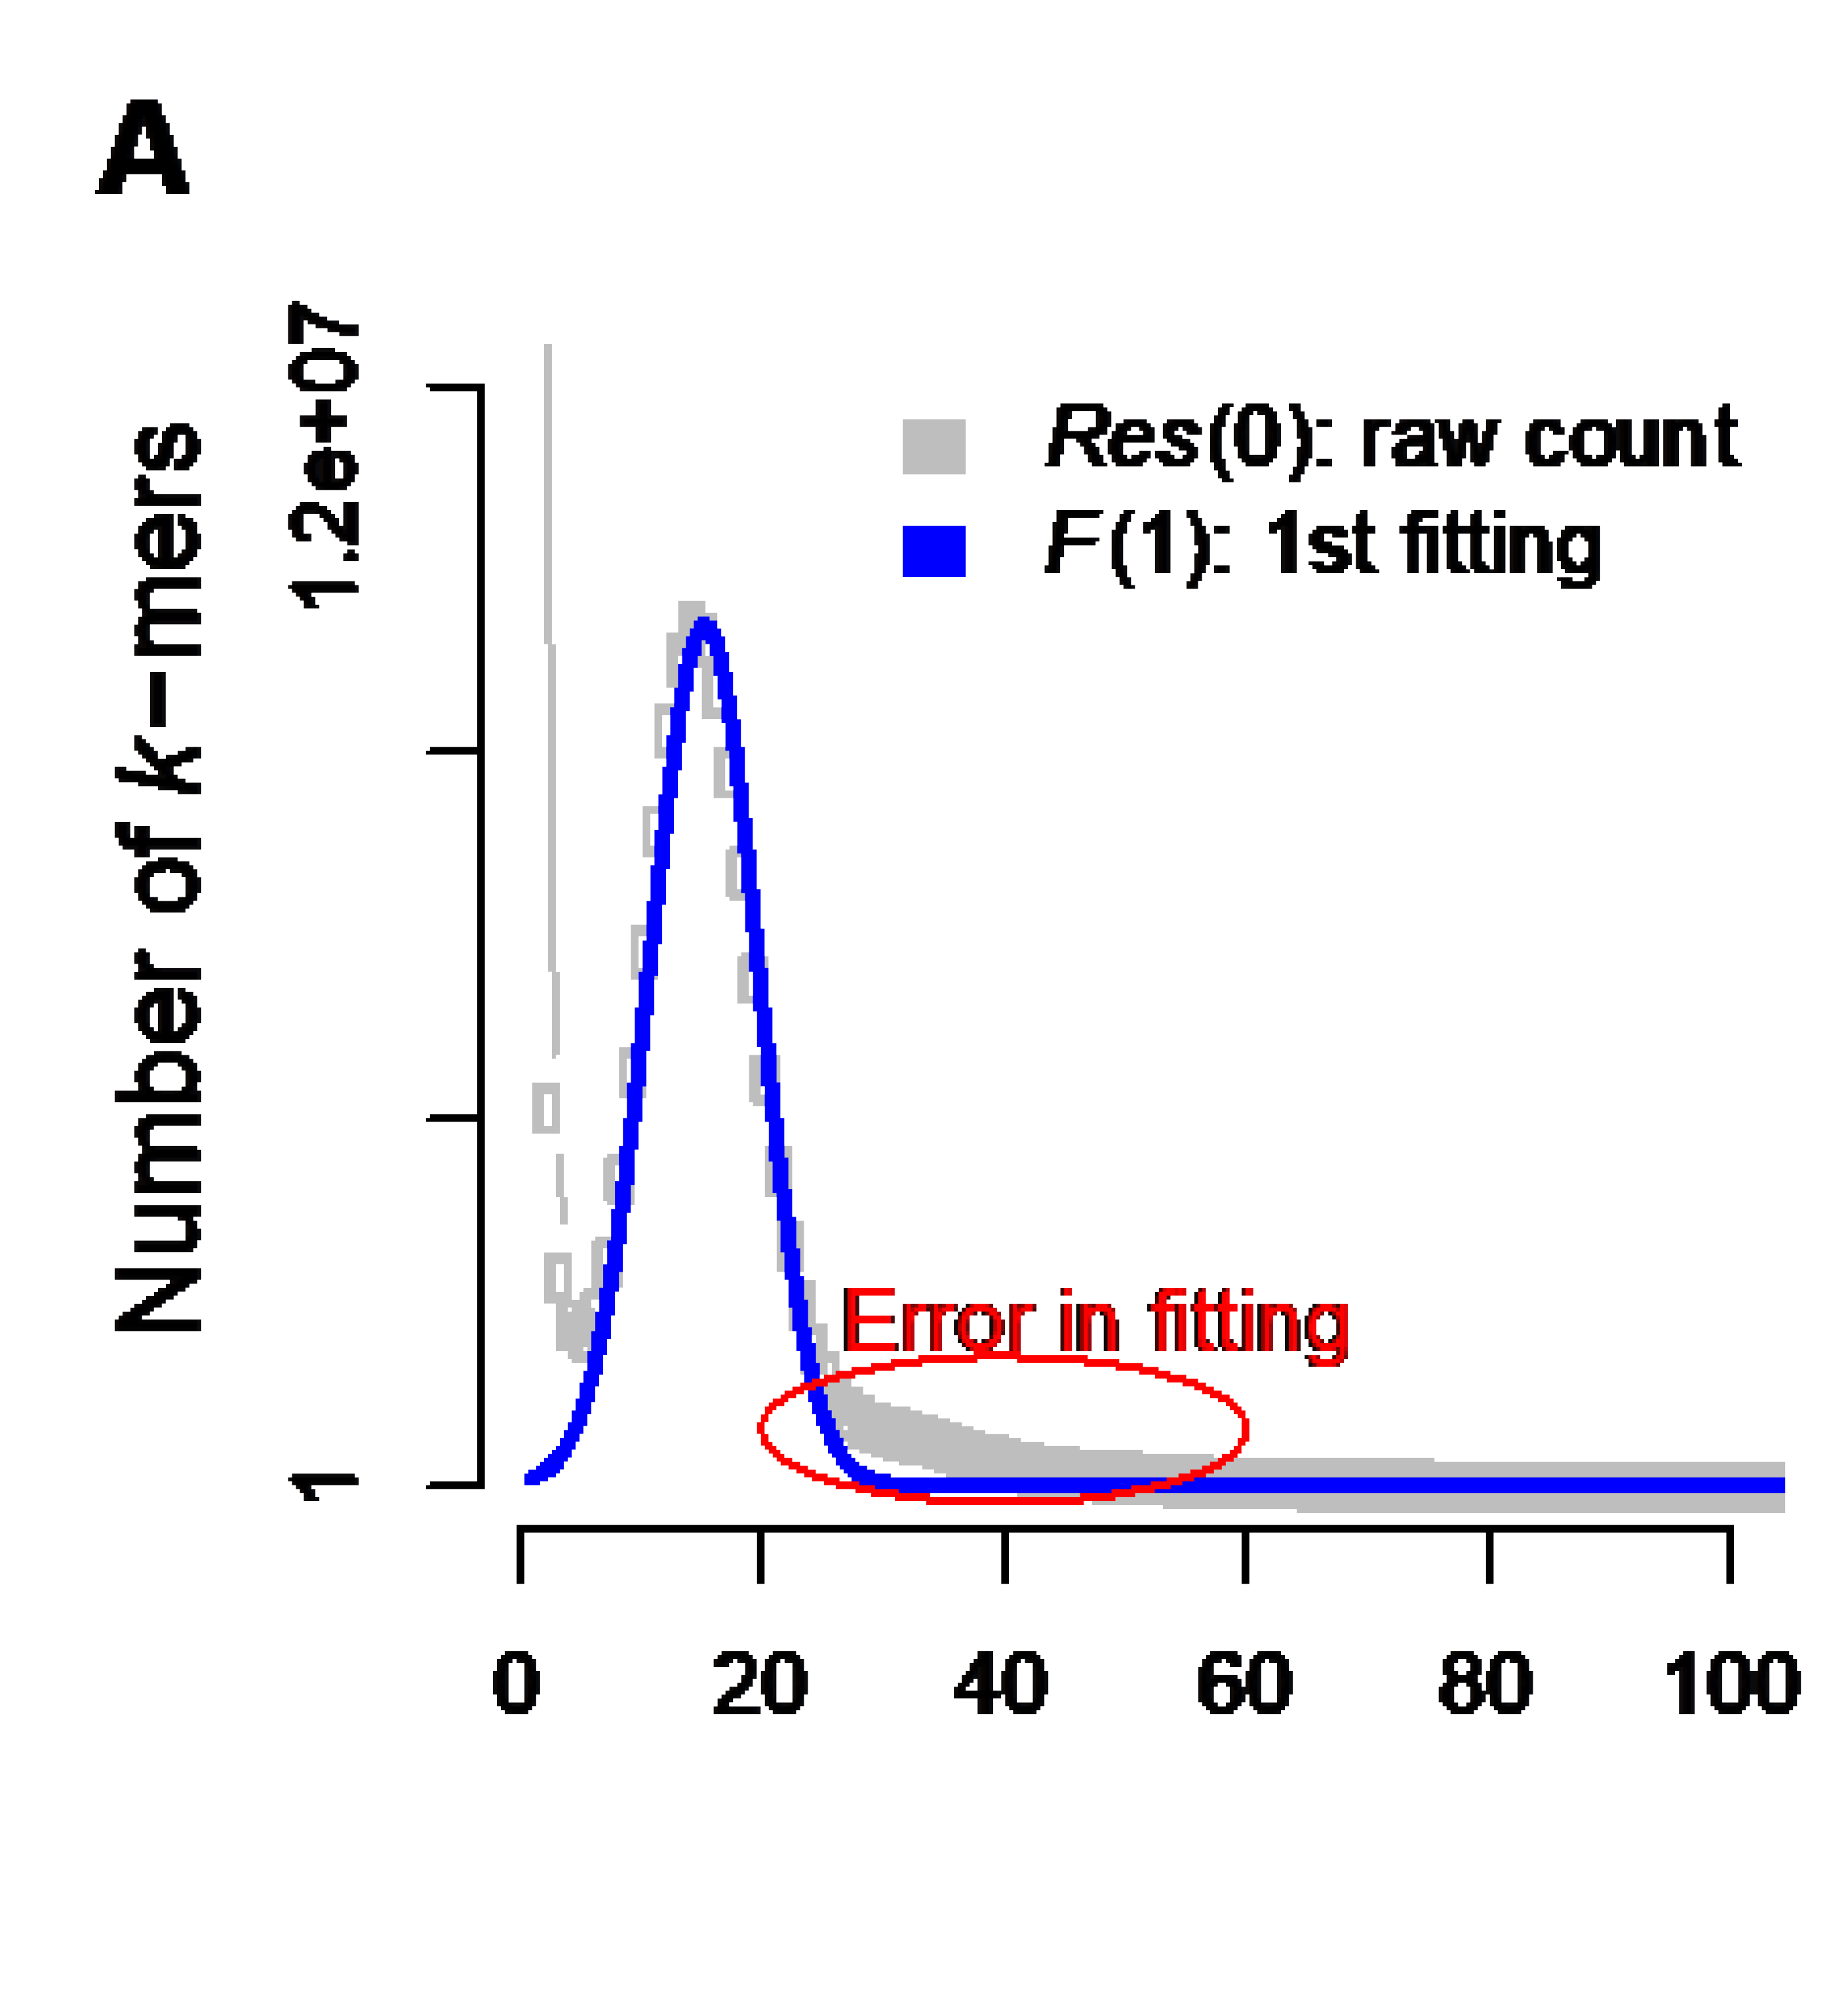
\includegraphics[width=0.31\textwidth]{capitoli/findGSE/fittingA.png}} \quad
		\subfloat[][\emph{Secondo fitting, utilizzando anche i k-mer residui dalla precedente operazione.}]
		{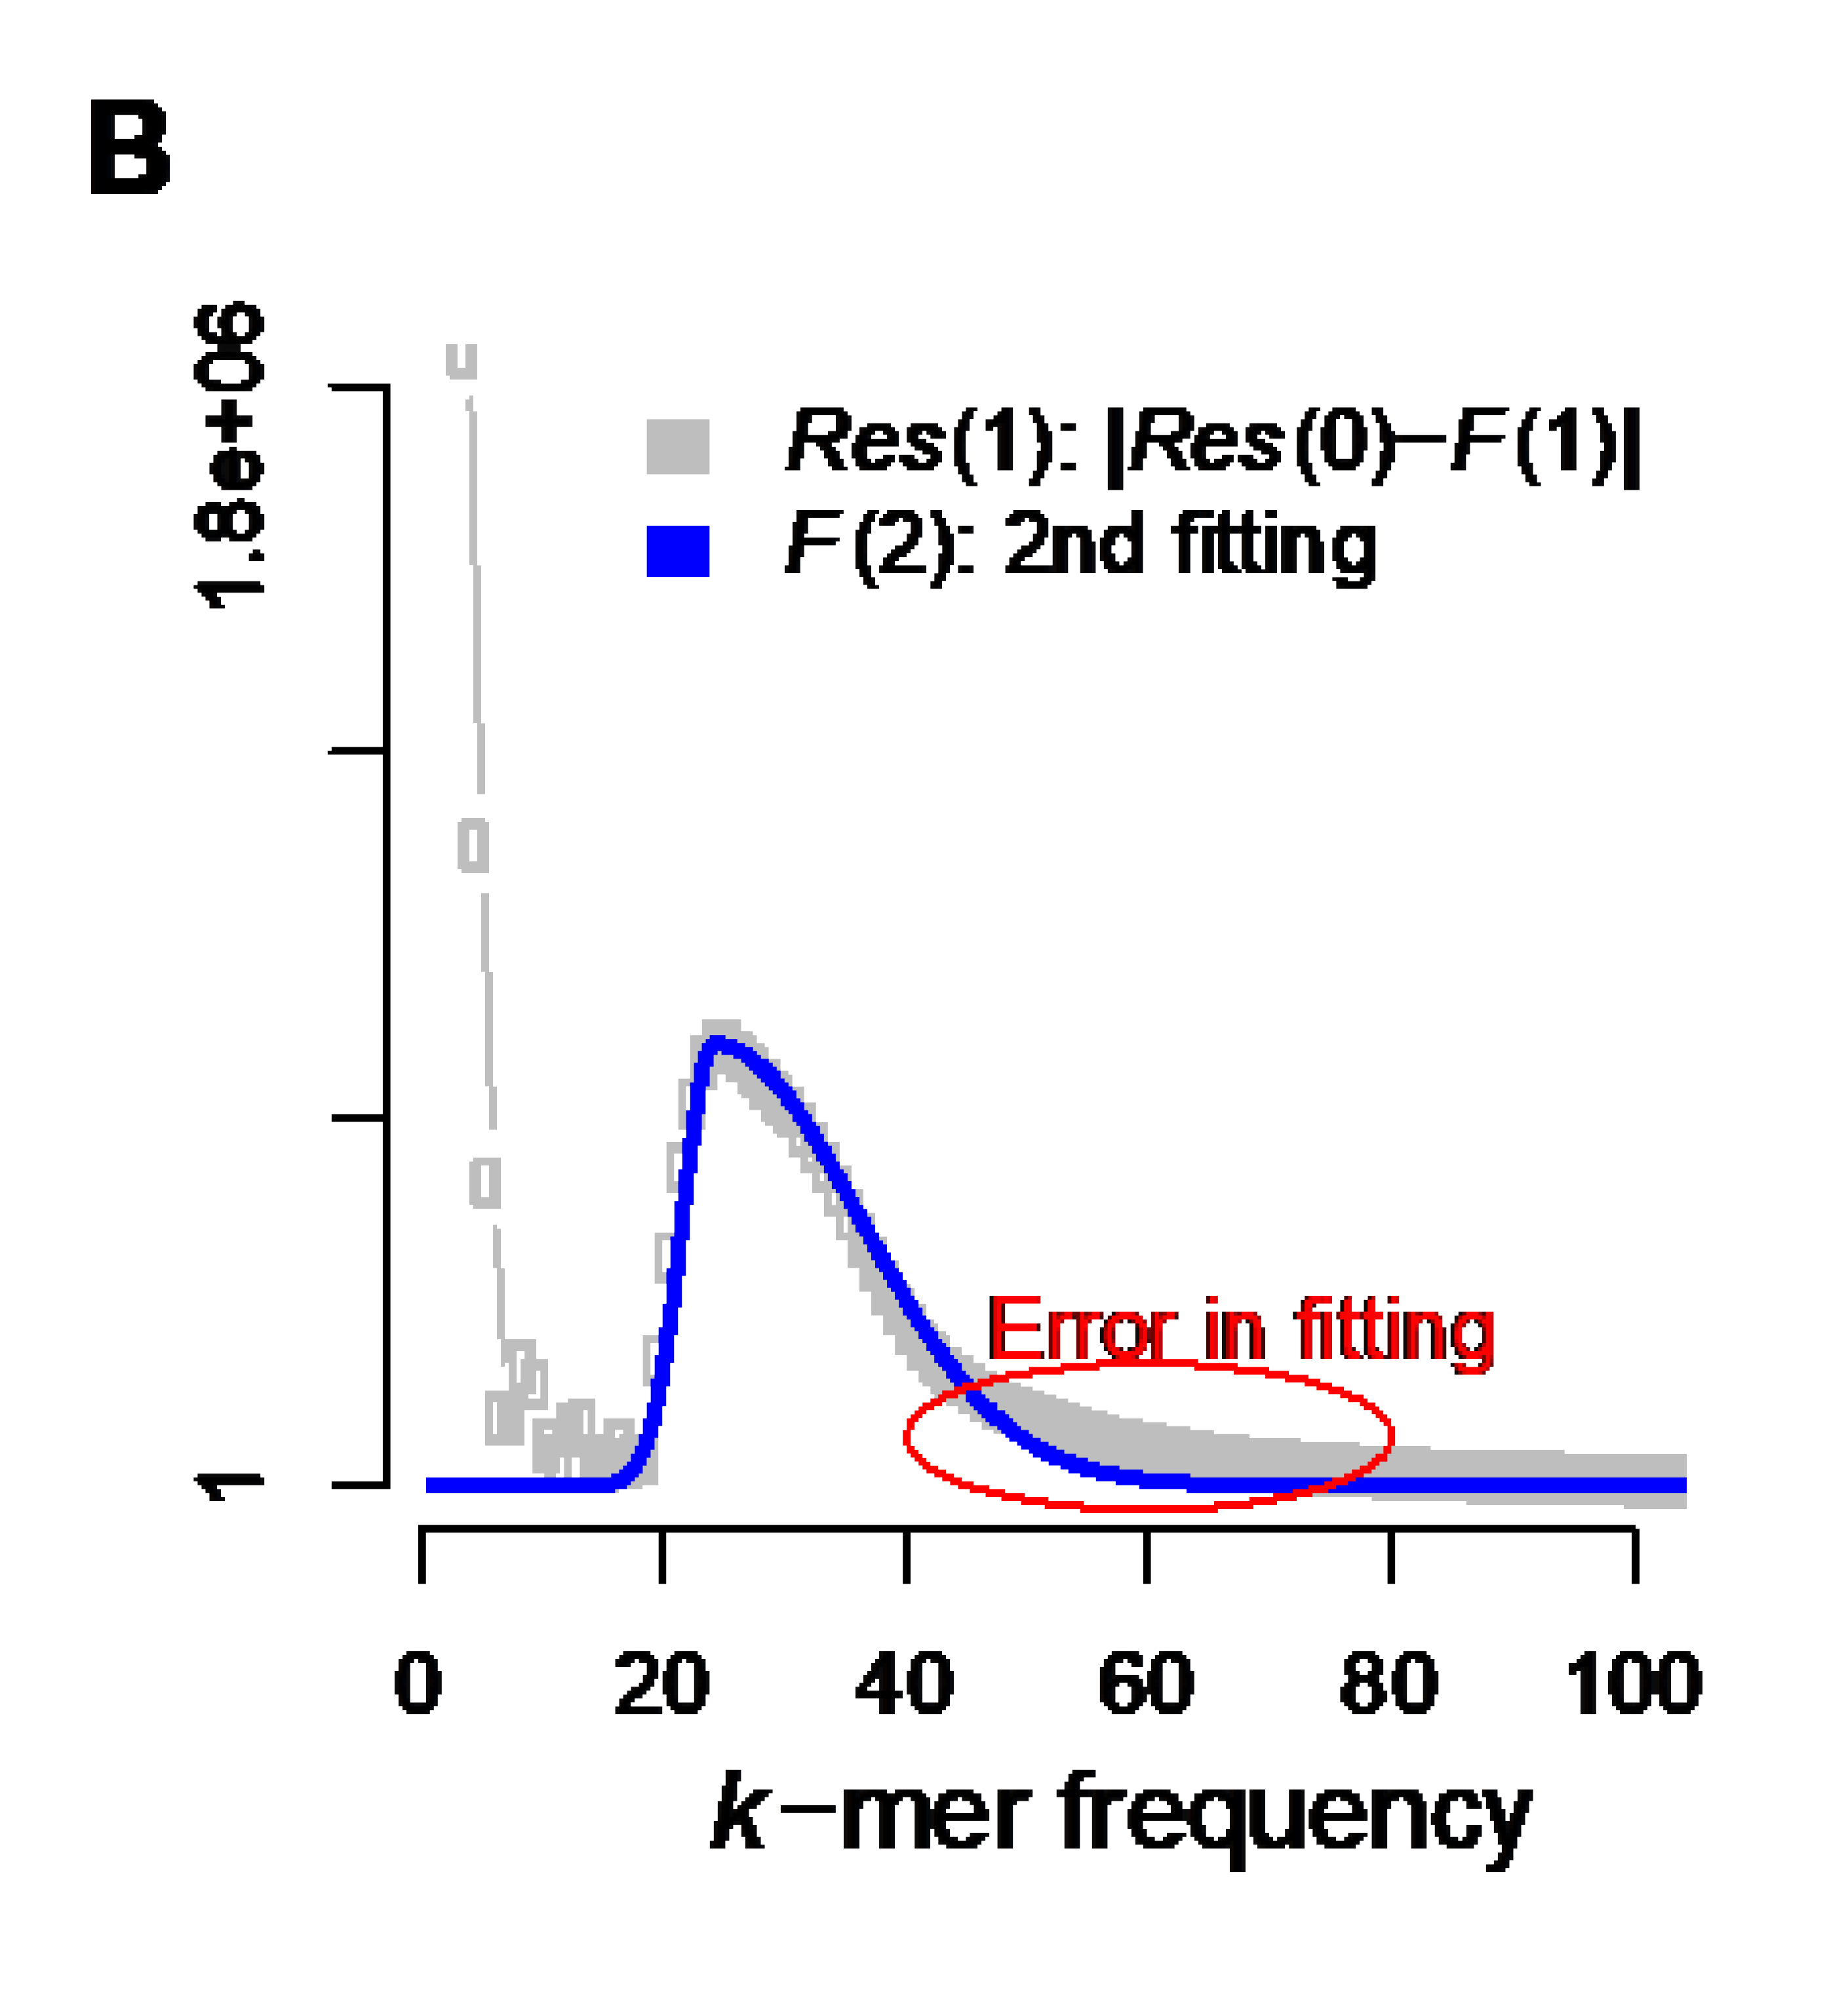
\includegraphics[width=0.31\textwidth]{capitoli/findGSE/fittingB.png}} \quad
		\subfloat[][\emph{Fitting finale.}]
		{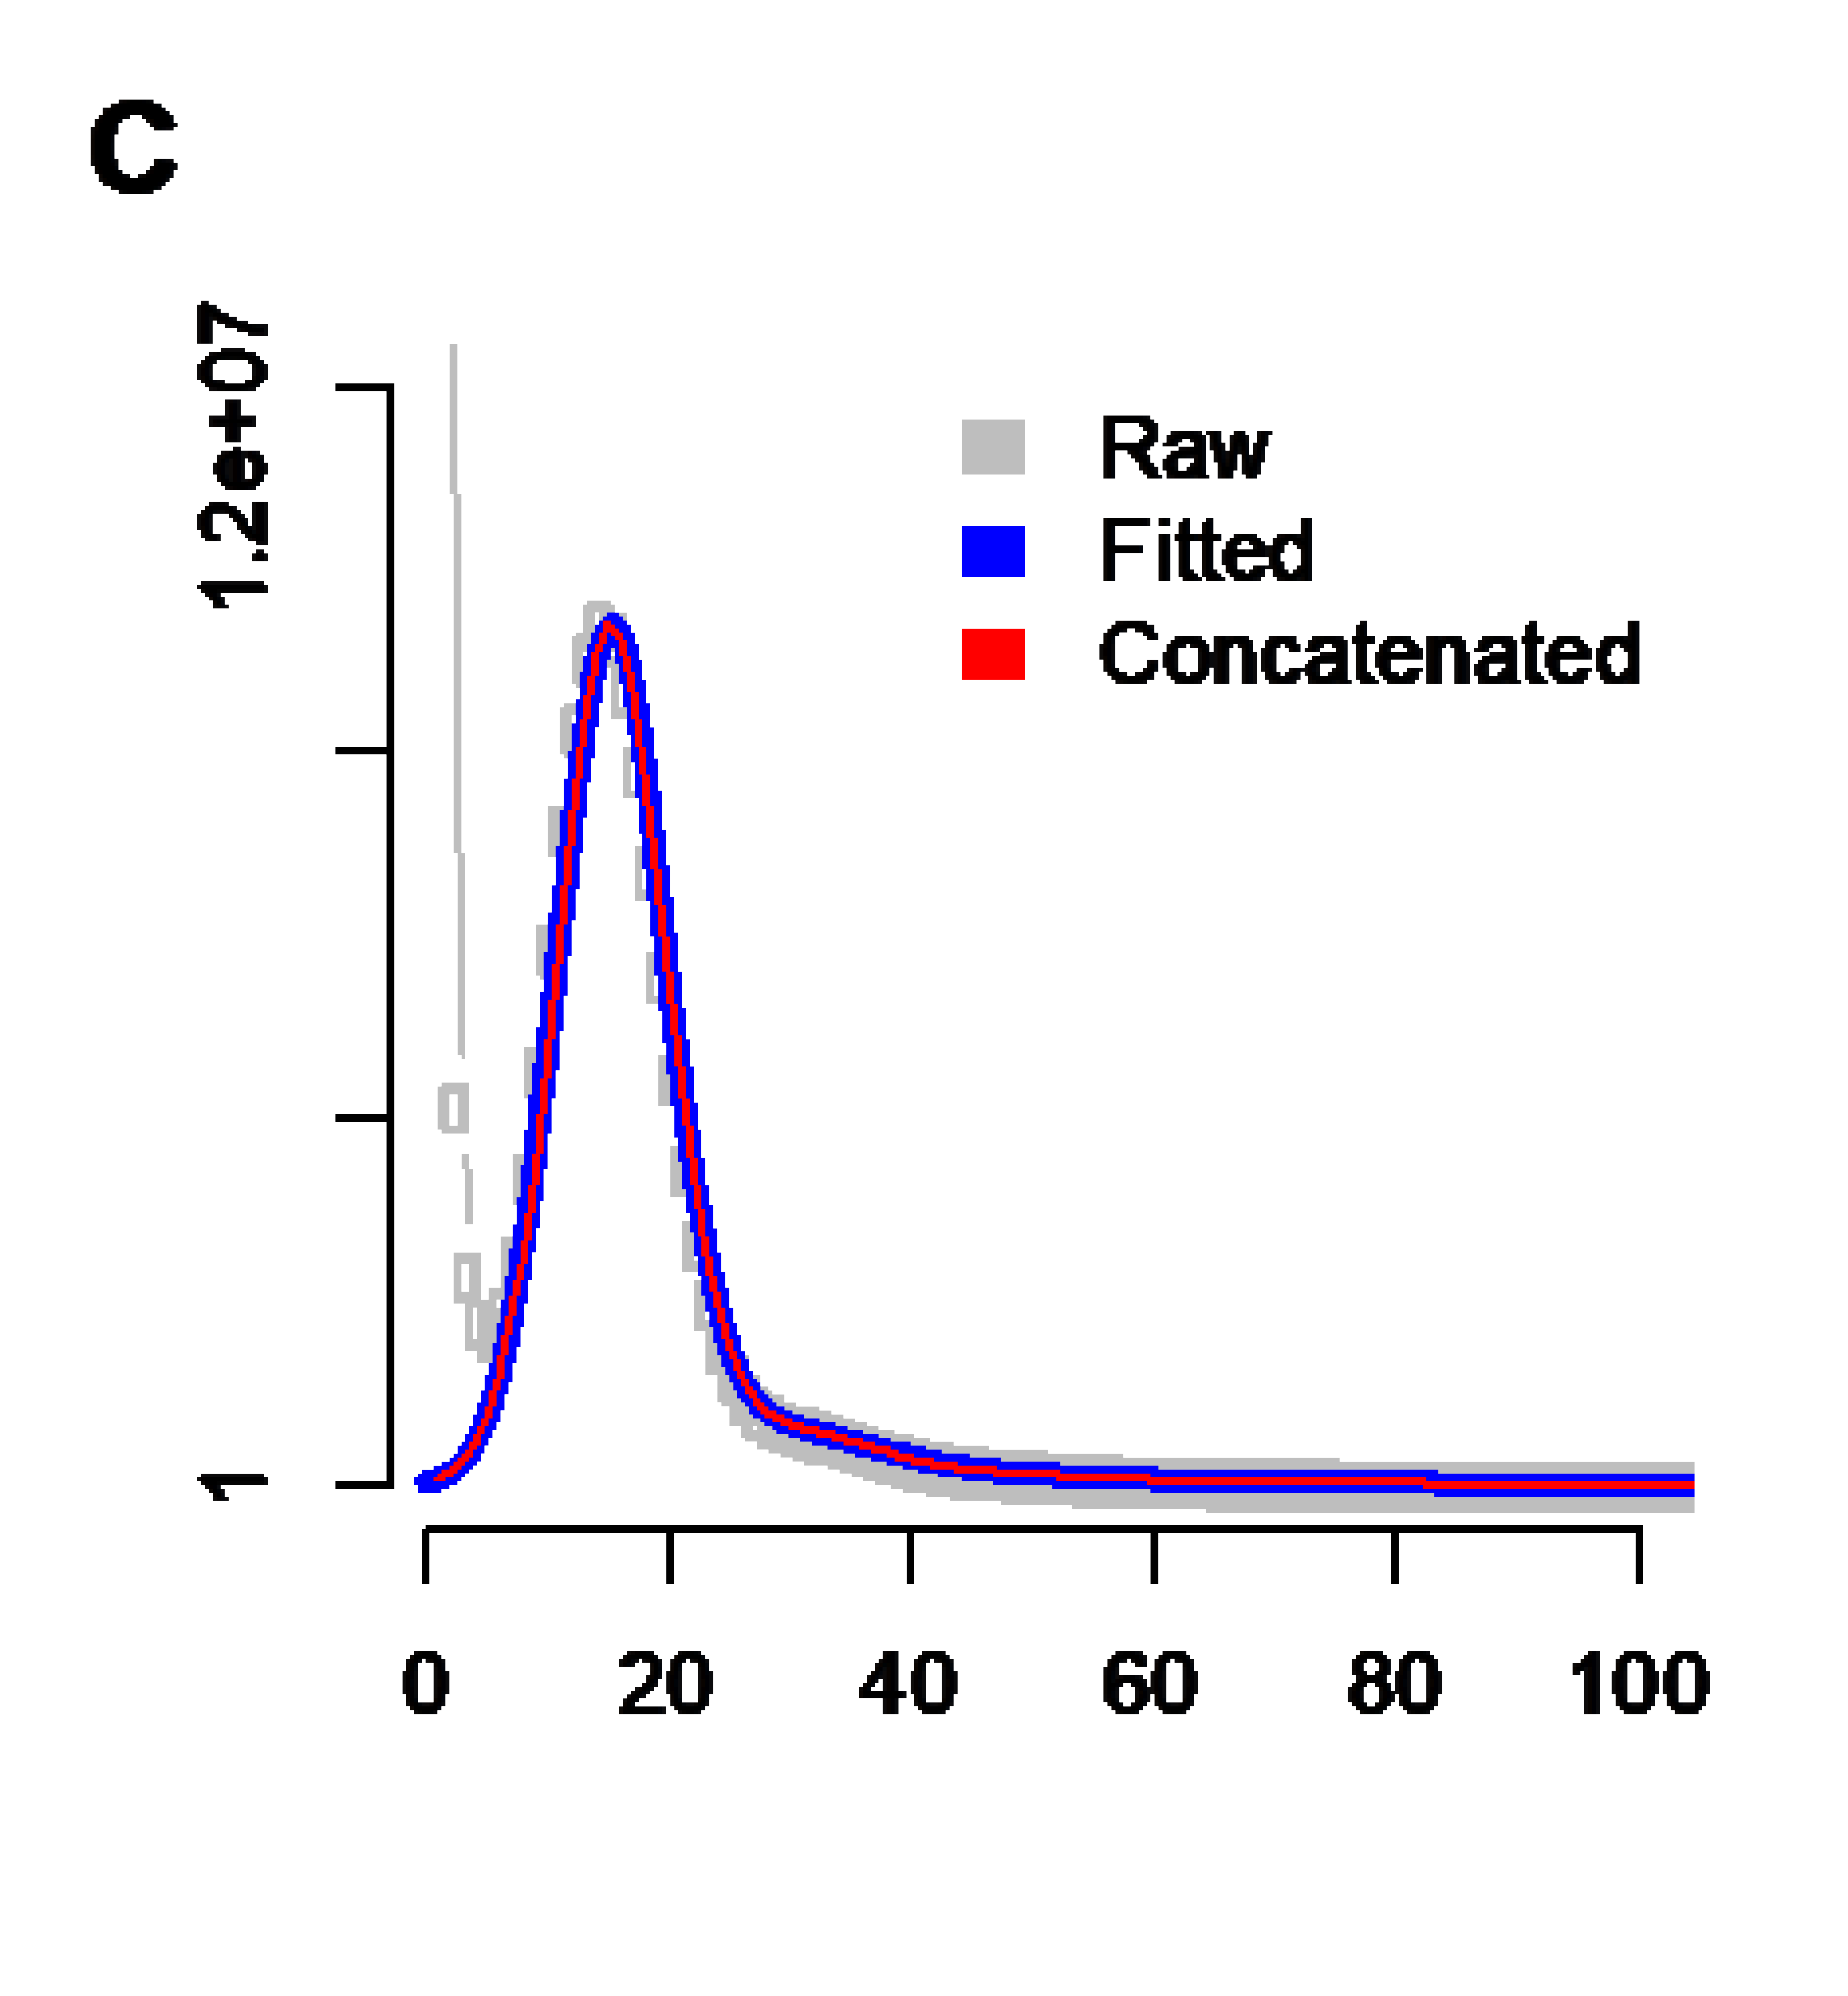
\includegraphics[width=0.31\textwidth]{capitoli/findGSE/fittingC.png}} 
		\caption{Esempio di fitting iterativo del k-mer profile.}
		\label{fig:findGSEfitting}
	\end{figure}


	Dato un genoma aploide con $G$ basi, il numero di k-mer possibili sarà $G-k+1$. Ponendo $C$ la copertura media dei k-mer, in modo che in media ogni k-mer sia trovato in $C$ letture diverse, e $N$ il numero di k-mer trovati nelle letture, la quantità di k-mer presenti nel genoma è descritta dall'equazione~\vref{eqn:findGSE1}. 	
	
	\begin{equation}
		\label{eqn:findGSE1}
		N=C \times (G-K+1).
	\end{equation}
		
	
	Posta la dimensione del genoma molto maggiore del numero di basi utilizzate $G\gg k$, l'equazione~\vref{eqn:findGSE2} approssima la dimensione totale del genoma in analisi.
	
	\begin{equation}
		\label{eqn:findGSE2}
		G\approx N/C.
	\end{equation}

	A partire sia dal profilo reale che dal modello stimato, il programma calcola quindi il numero totale di k-mer trovati $N$ e la copertura media dei k-mer $C$, per poi calcolare la dimensione del genoma attraverso l'equazione~\vref{eqn:findGSE2}.
	
	
	\subsection{Analisi di genomi reali}
	Utilizzando letture reali, i dati devono essere precedentemente processati per minimizzare gli errori di stima del genoma. Per questo è consigliabile ridurre prima le letture con il programma \textit{Skewer}~\cite{jiang2014skewer}, ed eliminare quelle con lunghezza minore di 33 bp. Per ottenere risultati migliori, inoltre, è consigliabile rimuovere le letture doppie dovute alla duplicazione PCR tramite il programma \textit{FastUniq}~\cite{xu2012fastuniq}, e le sequenze di simili a DNA dei mitocondri o dei cloroplasti con i programmi \textit{BWA}~\cite{li2009fast} e \textit{SAMtools}~\cite{li2009sequence}.
\end{document}